% This is the chapter 'Modeling' to the "Hodgkin-Huxley neuron model V2.0 book"
% Last edited 2026.08.08

\ifx\magyar\undefined
\chapter[Electrical model]{Electrical model\label{ch:Modell-electrical}}
\else
\chapter[Elektromos modell]{Elektromos modell\label{ch:Modell-electrical}}
\fi
\iflatexml
\else
\minitoc
\fi

\ifx\magyar\undefined

%
\else
%
Tisztán elektromos modellünkben a jelenségek
csupán a membrán felületén található elektrolit réteget érintik. A töltések taszító hatása következtében az ionok
a membrán felületén levő rétegben helyezkednek el. 
A felület durva (nem sík), ezért egy véges vatagságú 
réteget tételezünk fel. 
A rétegen belül a só molekulák nem ionizáltak.
\fi

\ifx\magyar\undefined
\section[Calculations]{Calculations in a cell\label{sec:V2-0_ElectricCalculations}}
\else
\section[Elektromos számítások]{Elektromos számítások\label{sec:V2-0_ElectricCalculations}}
\fi

\ifx\magyar\undefined
In this section, we only use our knowledge of the neuron to the extent that we perform calculations for the ions of the 'layer of life' as if they were point charges located in a lifeless medium. In the calculations, we use the disciplinary formulas of technical electricity, although we keep in mind the different properties of discrete electric charge carriers, especially their slowness.

%
\else
%
Ebben a szakaszban csupán annyit használunk
a neuronra vonatkozó ismeretekből, hogy az 'élet rétege' ionjaira vonatkozólag úgy végzünk számításokat, mintha azok egy élettelen közegben elhelyezkedő pontszerű töltések lennének. A számításokban a technikai elektromosságtan diszciplináris
formuláit használjuk, bár szem előtt tartjuk a diszkrét elektromos töltéshordozók eltérő tulajdonságait, főként lassúságukat.

Az erőhatások kiszámtásakor teljes mértékban a 
diszciplináris módszereket használjuk, és a módszereket
olyan fizikai elemre alkalmazzuk, amelynek paraméterei
megegyeznek aa fiziológiai mérések eredményével.
Természetesen az így származtatott értékek 
inkább nagyságrendi becslésként, mint pontos értékként
tekintendők
\fi



\ifx\magyar\undefined
\physicspanel{phys:CellForceinField}{Estimating the force exerted on ions in electric field}
{ By using that in an electric field $\vec F = q \vec E$, one can calculate the force exerted on a charge, that enables one to calculate also the particle's impulse, pressure, and energy. For example, in the case of $Na^+$ rush-in, the electric force field is $10^7$ [V/m].
 Since($[N/C]==[V/m]$),
the value of the force exerted on a single ion, accelerating it across the ion channel, is
\begin{equation}
	F_{Na^+}= 10^7  [N/C] \times 1.602* 10^{-19} [C] = %1.6*10^{-12}\ [N] 
	\SI{1.6e-12}{\newton}
	\label{eq:UnitForce}
\end{equation}

(Here we used data from Johnston\&Wu constants from \textbf{\hyperlink{num:JohnstonConstants}{Numerics panel~\ref{num:JohnstonConstants}}})
}

\else

\physicspanel{phys:CellForceinField}{Estimating the force exerted on ions in electric field}
{ By using that in an electric field $\vec F = q \vec E$, one can calculate the force exerted on a charge, that enables one to calculate also the particle's impulse, pressure, and energy. For example, in the case of $Na^+$ rush-in, the electric force field is $10^7$ [V/m].
 Since($[N/C]==[V/m]$),
the value of the force exerted on a single ion, accelerating it across the ion channel, is
\begin{equation}
	F_{Na^+}= 10^7  [N/C] \times 1.602* 10^{-19} [C] = %1.6*10^{-12}\ [N] 
	\SI{1.6e-12}{\newton}
	\label{eq:UnitForce}
\end{equation}

(Here we used data from Johnston\&Wu constants from \textbf{\hyperlink{num:JohnstonConstants}{Numerics panel~\ref{num:JohnstonConstants}}})
}

\fi


\ifx\magyar\undefined
\physicspanel{phys:CellAccelerationinField}{Estimating the acceleration of ions in electric field}
{
The force in the ion channel was calculated in
\textbf{\hyperlink{phys:CellForceinField}{Physics Panel~\ref{phys:CellForceinField}}}
\noindent
and the mass of a $Na^+$ ion is $m_{Na} = 3.82\times 10^{-26}\ kg$.
It causes an acceleration
\begin{equation}
a=\frac{F_{Na^+}}{m_{Na^+}} = \frac{1.6*10^{-12}\ [N]}{ 3.82\times 10^{-26}\ [kg]} =
0.42 \times 10^{14}\ [\frac{m}{s^{2}}]
\label{eq:Physics-RushInAceleration}
\end{equation}
\noindent
The distance $d$ to travel (without collision) is the thickness of the neuronal membrane $5*10^{-9}\ nm$
and we assume a continuosly accelerating ion. Using $d=\frac{1}{2}\times a\times t^2$
\begin{equation}
t_{traverse} = \sqrt{\frac{2\times 5*10^{-9} [m]}{0.42\times 10^{14} [\frac{m}{s^{2}}]}} = 1.54\times 10^{-11}\ [s]
\end{equation}

However, the mean free path (the distance an ion travels without collision) is very small, about
\SI{2\times 10e-10}{\meter}. In the collision the
ion loses its energy, then starts to accelerate again.
This way, the traverse time is
%
\begin{equation}
t_{traverse} = \frac{5}{0.2}\sqrt{\frac{2\times 2*10^{-10} [m]}{0.42\times 10^{14} [\frac{m}{s^{2}}]}} = 25\times 3\times 10^{-13}\ = 7.5\times 10^{-11}\ [s]
\end{equation}
%
That is, the time is higher, but the order of our estimation remains unchanged.
}

\else

\physicspanel{phys:CellAccelerationinField}{Estimating the acceleration of ions in electric field}
{
The force in the ion channel was calculated in
c\noindent
and the mass of a $Na^+$ ion is $m_{Na} = 3.82\times 10^{-26}\ kg$.
It causes an acceleration
\begin{equation}
a=\frac{F_{Na^+}}{m_{Na^+}} = \frac{1.6*10^{-12}\ [N]}{ 3.82\times 10^{-26}\ [kg]} =
0.42 \times 10^{14}\ [\frac{m}{s^{2}}]
\label{eq:Physics-RushInAceleration}
\end{equation}
\noindent
The distance $d$ to travel (without collision) is the thickness of the neuronal membrane $5*10^{-9}\ nm$
and we assume a continuosly accelerating ion. Using $d=\frac{1}{2}\times a\times t^2$
\begin{equation}
t_{traverse} = \sqrt{\frac{2\times 5*10^{-9} [m]}{0.42\times 10^{14} [\frac{m}{s^{2}}]}} = 1.54\times 10^{-11}\ [s]
\end{equation}

Az ionok közepes szabad úthossza azonban igen kicsi,
pl. \SI{2\times 10e-10}{meter}. Az ion ekkora utat tesz meg, aztán egy ütközésben elveszti az addig szerzett
energiát, és újból felgyorsul. Ilyen módon az áthaladási idő

\begin{equation}
t_{traverse} = \frac{5}{0.2}\sqrt{\frac{2\times 2*10^{-10} [m]}{0.42\times 10^{14} [\frac{m}{s^{2}}]}} = 25\times 3\times 10^{-13}\ = 7.5\times 10^{-11}\ [s]
\end{equation}
azaz az idő valamivel magasabb, de becslésünk nagyságrendje változatlan marad.
}
\fi


\ifx\magyar\undefined
The acceleration of an ion is unbelievably large,
see \textbf{\hyperlink{phys:CellAccelerationinField}{Physics Panel~\ref{phys:CellAccelerationinField}}}.
It is sufficiently large to keep the potential at the same value
over an extended object,
provided that the ions must follow a small and slow change, such as due to the
"leaking" current through the
\gls{AIS}.
Similarly, the ions can 'instantly' follow quick changes such as
a square wave gradient.
%
\else
%
Az ionok gyorsulása hihetetlenül nagy, lásd 
\textbf{\hyperlink{phys:CellAccelerationinField}{Physics Panel~\ref{phys:CellAccelerationinField}}}.
Elég gyors ahhoz, hogy a potenciált egy kiterjedt objektumon azonos értéken tartsa,
feltéve, hogy az ionoknak kis és lassú változásokat kell követniük, mint amilyen például az \gls{AIS}
szivárgó árama.

Similarly, the ions can 'instantly' follow quick changes such as
a square wave gradient.
\fi

\ifx\magyar\undefined
\physicspanel{phys:CellIonDensity}{Ion density and force on membrane's surface}
{
Using data from 
\textbf{\hyperlink{num:JohnstonConstants}{Numerics panel~\ref{num:JohnstonConstants}}}), and assuming that 
the electrical repulsion keeps the surface density of ions uniform, one can calculate the area an ion occupies, and the distance between ions as the square root of that area
\[
D_{ions} = \sqrt{\frac{8\times 10^{-9}}{10^7}} = 2.8\times 10^{-8}\ m
\]

That is, the average distance between ions on the surface
is about 150 times larger than the ion's diameter.
Applying the formula
\[
F_{ions}= \frac{1}{4\pi\epsilon_\circ}\frac{q^2}{r^2}
\]
using the elementay charge and the distance calculated,
results in
\[
F_{ions}= \SI{2.9e-13}{\newton}
\]
By comparing that value to the force acting across
the membran as given in \textbf{\hyperlink{phys:CellForceinField}{Numerics panel~\ref{phys:CellForceinField}}}),
one can see that the force perpendicular to the membrane is an order of magnitude larger than
the force among the ions on the surface.
}
%
\else
%
\physicspanel{phys:CellIonDensity}{Ion sűrűség és erő a membrán felületén}
{
Using data from 
\textbf{\hyperlink{num:JohnstonConstants}{Numerics panel~\ref{num:JohnstonConstants}}}), and assuming that 
the electrical repulsion keeps the surface density of ions uniform, one can calculate the area an ion occupies, and the distance between ions as the square root of that area
\[
D_{ions} = \sqrt{\frac{8\times 10^{-9}}{10^7}} = 2.8\times 10^{-8}\ m
\]

That is, the average distance between ions on the surface
is about 150 times larger than the ion's diameter.
Applying the formula
\[
F_{ions}= \frac{1}{4\pi\epsilon_\circ}\frac{q^2}{r^2}
\]
using the elementay charge and the distance calculated,
results in
\[
F_{ions}= \SI{2.9e-13}{\newton}
\]
By comparing that value to the force acting across
the membran as given in \textbf{\hyperlink{phys:CellForceinField}{Numerics panel~\ref{phys:CellForceinField}}}),
one can see that the force perpendicular to the membrane is an order of magnitude larger than
the force among the ions on the surface.
}
\fi


\ifx\magyar\undefined
\physicspanel{phys:CellAccelerationinField}{Estimating the acceleration of ions in electric field}
{
The force in the ion channel was calculated in
\textbf{\hyperlink{phys:CellForceinField}{Physics Panel~\ref{phys:CellForceinField}}}
\noindent
and the mass of a $Na^+$ ion is $m_{Na} = 3.82\times 10^{-26}\ kg$.
It causes an acceleration
\begin{equation}
a=\frac{F_{Na^+}}{m_{Na^+}} = \frac{1.6*10^{-12}\ [N]}{ 3.82\times 10^{-26}\ [kg]} =
0.42 \times 10^{14}\ [\frac{m}{s^{2}}]
\label{eq:Physics-RushInAceleration}
\end{equation}
\noindent
The distance $d$ to travel (without collision) is the thickness of the neuronal membrane $5*10^{-9}\ nm$
and we assume a continuosly accelerating ion. Using $d=\frac{1}{2}\times a\times t^2$
\begin{equation}
t_{traverse} = \sqrt{\frac{2\times 5*10^{-9} [m]}{0.42\times 10^{14} [\frac{m}{s^{2}}]}} = 1.54\times 10^{-11}\ [s]
\end{equation}

The acceleration of an ion is unbelievably large. It is sufficiently large to keep the potential at the same value
over an extended object,
provided that the ions must follow a small and slow change, such as due to the
"leaking" current through the
\gls{AIS}.
Similarly, the ions can 'instantly' follow quick changes such as
a square wave gradient.
}

\else

\physicspanel{phys:CellAccelerationinField}{Estimating the acceleration of ions in electric field}
{
The force in the ion channel was calculated in
\textbf{\hyperlink{phys:CellForceinField}{Physics Panel~\ref{phys:CellForceinField}}}
\noindent
and the mass of a $Na^+$ ion is $m_{Na} = 3.82\times 10^{-26}\ kg$.
It causes an acceleration
\begin{equation}
a=\frac{F_{Na^+}}{m_{Na^+}} = \frac{1.6*10^{-12}\ [N]}{ 3.82\times 10^{-26}\ [kg]} =
0.42 \times 10^{14}\ [\frac{m}{s^{2}}]
\label{eq:Physics-RushInAceleration}
\end{equation}
\noindent
The distance $d$ to travel (without collision) is the thickness of the neuronal membrane $5*10^{-9}\ nm$
and we assume a continuosly accelerating ion. Using $d=\frac{1}{2}\times a\times t^2$
\begin{equation}
t_{traverse} = \sqrt{\frac{2\times 5*10^{-9} [m]}{0.42\times 10^{14} [\frac{m}{s^{2}}]}} = 1.54\times 10^{-11}\ [s]
\end{equation}

The acceleration of an ion is unbelievably large. It is sufficiently large to keep the potential at the same value
over an extended object,
provided that the ions must follow a small and slow change, such as due to the
"leaking" current through the
\gls{AIS}.
Similarly, the ions can 'instantly' follow quick changes such as
a square wave gradient.
}

\fi


\ifx\magyar\undefined
\section[Method of electrical description]{Method of electrical description\label{sec:V2-0_ElectricLanguage}}
\else
\section[Az elektromos leírás módja]{Az elektromos leírás módja\label{sec:V2-0_ElectricLanguage}}
\fi


\ifx\magyar\undefined
An essential element of our electrical model is that inside the insulating sphere shown in Figure~\ref{fig:LipidSphere}, in direct contact with it, there is a nanometer-thick electrolyte layer, see section~\ref{sec:AbstractLayer}. We consider the layer ('layer of life') to be homogeneous, and within this the interior of the neuron ('bulk') is also homogeneous. This layer is responsible for the electrical phenomena. The ions that create the resting potential are located in the layer shown in Figure~\ref{fig:MembraneSurface} on the surface of the neuron; these are held firmly in place in the resting state by the opposite charges on the other side of the membrane. The $Na^+$ ions that flow in at the beginning of the action potential "stop" in this layer and leave from there through the \gls{AIS}. In other words, this layer essentially forms the capacitor in the electrical description. Note that ions form a 'slow' current, which can be ignored for some phenomena.

Our electrical model describes the neuron as a circuit in which charges are present, voltages can arise and currents can flow, and we use concepts known from technical electricity. In the resting state, the intracellular and extracellular potentials of the neuron (in other words, the electrolyte potential on the inner and outer sides of the neuron membrane) are the same, so there is no potential difference that would drive current through the membrane. However, the voltage of the neuron is composed of one electrostatic and two thermodynamic (Nernst) voltages. Figure~\ref{fig:RestingPotential3} graphically summarizes the formation of the potential,
%\textbf
{\hyperlink{phys:ElectricModel}{\ref{phys:ElectricModel} physics panel}}
describes the mathematics of the voltage relations, and Table~\ref{Tab:SummaryTable} compares the theoretical 
results to the measured values.
%
\else
%
Elektromos modellünk lényeges eleme, hogy a \ref{fig:LipidSphere}~ábra szerinti szigetelő gömbön belül, vele közvetlenül érintkezve, egy nanométer vastagságú elektrolit réteg helyezkedik el, lásd \ref{sec:AbstractLayer}~szakasz. A réteget ('az élet rétege') homogénnek tekintjük,  ezen belül a neuron belsejét ('bulk') szintén homogénnek. Az elektromos jelenségekért ez a réteg felelős. A neuron felszínén, lásd \ref{fig:MembraneSurface}~ábra, levő rétegben helyezkednek el azok az ionok, amelyek a nyugalmi potenciált (lásd \ref{sec:Model-NeuronAbstractResting}~szakasz)  hozzák létre; ezeket a membrán másik oldalán levő ellentétes töltések szilárdan a helyükön tartják nyugalmi állapotban. Az akciós potenciál (lásd \ref{sec:Model-NeuronAbstractAction}~szakasz) kezdetekor beözönlő $Na^+$ ionok ebben a rétegben "megállnak", és innét távoznak az \gls{AIS}-en keresztül.  Azaz, lényegében ez a réteg alkotja az elektromos leírásban a kondenzátort. Megjegyezzük, hogy az ionok 'lassú' áramot alkotnak, ami a jelenségek egy részénél figyelmen kívül hagyható.

Elektromos modellünk a neuront olyan áramkörként írja le, amelyikben töltések vannak jelen, feszültségek 
keletkezhetnek és áramok folyhatnak, és
a technikai elektromosságtanból ismert fogalmakat használjuk.
A nyugalmi állapotban 
a neuron intracelluláris és extracelluláris potenciálja 
(másként a neuron membrán belső és külső oldalán az
elektrolit potenciálja) azonos,
így nincs olyan potenciálkülönbség, ami áramot hajtana át a membránon. 
A neuron feszültsége azonban egy elektrosztatikus és két termodinamikus (Nernst) feszültségből tevődik össze.
A \ref{fig:RestingPotential3}.~ábra képszerűen foglalja össze
a potenciál kialakulását, a
{\hyperlink{phys:ElectricModel}{\ref{phys:ElectricModel} physics panel}} 
pedig a potenciálviszony összefüggését adja meg,
a~\ref{Tab:SummaryTable} táblázat pedig összehasonlítja az elméleti és a kísérleti adatokat.
\fi

\ifx\magyar\undefined
Electric charges accumulate on both sides of the membrane,
which create a potential difference.
The orange arrow in the middle indicates the capacitor voltage.
So, contrary to the assumption of \gls{HH}, the potential difference is not created by a constantly flowing current, the "leakage current", but by charges attached to the membrane.
Essentially, according to Kirchoff's voltage rule:
by adding the sum of the Nernst voltages of the ions on both sides of the membrane to the voltage on the capacitor between them,
we get zero voltage. The names of the ions that create the Nernst voltages are only shown on one side.
The curved arrows on both sides of the figure indicate the Nernst voltage of the two ions: the difference in the voltage coordinates of the end points corresponds to the Nernst voltage. The zero point is marked at the
zero voltage value on both the outer and inner sides. Following the arrows between the two zero points, we obtain a circuit where no current flows.
%
\else
%
A membrán két oldalán elektromos töltések halmozódnak fel,
amelyek potenciálkülönbséget hoznak létre.
Középütt a narancssárga nyíl jelöli a kondenzátor feszültséget. 
Tehát \gls{HH} feltételezésével ellentétben, a potenciál különbséget nem egy állandóan folyó áram, a "leakage current" hozza létre, hanem a membránra tapadt töltések.
Lényegében Kirchoff feszültség szabálya alapján:
a membrán két oldalán az ionok Nernst-feszültségeinek összegét a közöttük elhelyezkedő kondenzátoron levő feszültséggel összeadva,
nulla feszültséget kapunk. A Nernst-feszültségeket létrehozó ionok nevét csak az egyik oldalon tüntettük fel.
Az ábra a két oldalán hajlított nyilak jelölik a a két-két ion Nernst-feszültségét: a végpontok feszültség koordinátáinak különbsége a Nernst feszültségnek felel meg. A nullpontot a külső és belső oldalon egyaránt a    
nulla feszültség értéknél jelöltük ki. A két nullpont között
a nyilak mentén haladva olyan áramkört kapunk, ahol nem folyik áram.
\fi

\ifx\magyar\undefined

\begin{figure}
\iflatexml
	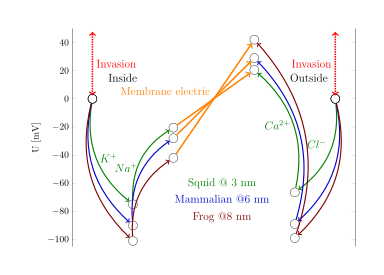
\includegraphics[width=.8\columnwidth]{fig/RestingPotential3.svg}
	\else
	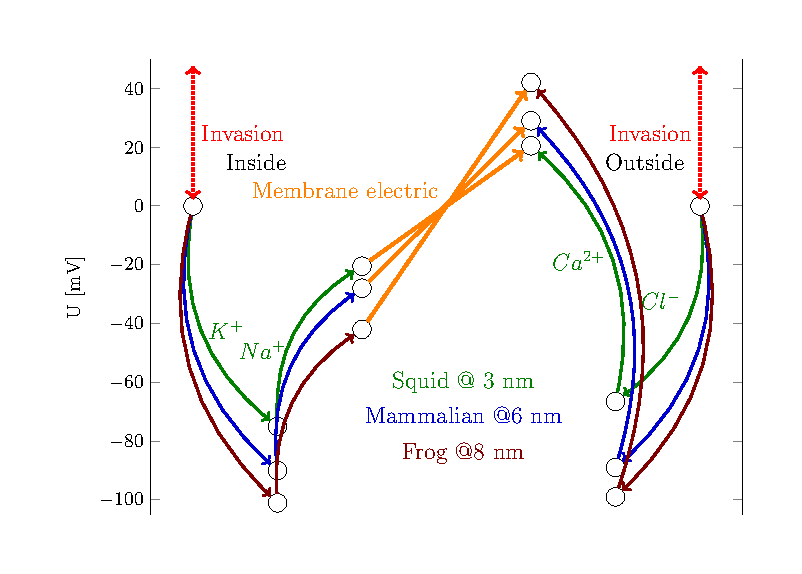
\includegraphics[width=.8\columnwidth]{fig/RestingPotential3.pdf}
\fi
	\caption{The mechanism for setting neuronal voltages is the same for all species shown in Table~\ref{Tab:SummaryTable}. It appears that 
		the thicker membrane produces a higher membrane electric potential and requires a higher thermal potential to compensate for it. However, it can solve the task using a lower salt concentration.
		Given that the electric membrane potential 
		accelerates the ions across the ion channels in the membrane, and the operation is faster. The electric field has a similar value, as shown in  Fig.~\ref{fig:NernstPlanckThermalWidth}.
		Furthermore, 
		the total concentration decreases as the membrane thickness and potential increase.  
		\label{fig:RestingPotential3}
	}
\end{figure}

\else

\begin{figure}
\iflatexml
	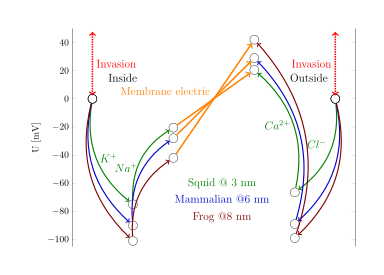
\includegraphics[width=.8\columnwidth]{fig/RestingPotential3.svg}
	\else
	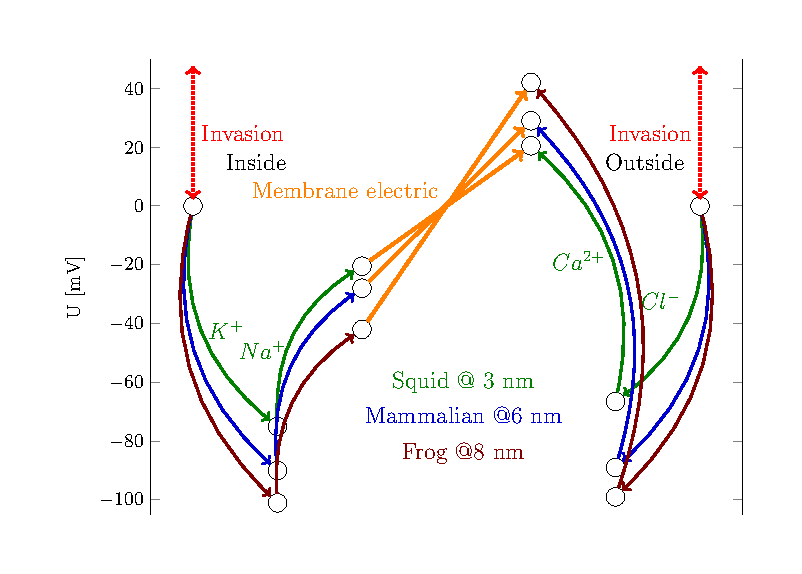
\includegraphics[width=.8\columnwidth]{fig/RestingPotential3.pdf}
\fi
	\caption{
A neuron potenciál viszonyainak kialakulása ugyanaz
három különböző faj esetén, az adatokat lásd
a~\ref{Tab:SummaryTable}~táblázatban.  
Úgy tűnik, a vastagabb membrán magasabb elektromos 
membrán feszültséget generál, amit csak nagyobb termodinamikus feszültség tud kompenzálni.	
A feladatot azonban alacsonyabb só-koncentrációval 
is meg lehet oldani.
Mivel az elektromos membrán feszültség gyorsítja az
ionokat a membránban levő ioncsatornán történő áthaladáskor, a működés emiatt gyorsabb.
Az elektromos tér azonban hasonló értékű, lásd még a~\ref{fig:NernstPlanckThermalWidth} ábrát.
Továbbá, a membrán vastagság és a potenciálkülönbség
növekedésével a teljes koncentráció csökken. 
		\label{fig:RestingPotential3}
	}
\end{figure}

\fi

\ifx\magyar\undefined

The electric voltage contribution is unidirectional, the two-component thermodynamic contributions, depending on the concentrations, can be positive or negative.
If choosing the zero potential at the middle of the electric potential, we can interpret that
the concentration combinations maintain their ionic concentrations (and so also thermodynamic voltage contributions) independently on both sides starting from a zero potential level. They generate potentials autonomously in the segments proximal to the opposite surfaces of the membrane. The electric charge on the membrane creates another voltage independently. However, that voltage must fit between the two thermodynamic voltages. Any deviation in the potentials starts a current directing the concentrations and voltages toward a balanced state.
The process is complex: the sum of surface concentration of ions must be the same on both sides for the condenser and the ratios on the intracellular and extracellular sides must be adjusted to satisfy the conditions the conditions shown in {\hyperlink{phys:ElectricModel}{\ref{phys:ElectricModel} physics panel}}.

\physicspanel{phys:ElectricModel}{Voltage relations in a neuron}
{
The local electric and concentration gradients control the local potentials:

\begin{tabular}{lllll}
$U_{internal}^{K^+,Na^+}$  & $= -U_{electric}$ & $+ U_{internal}^{K^+} $ & $+ U_{internal}^{Na^+}$ & $(+U_{internal}^{invasion})$\\
$U_{external}^{Cl^-,Ca^{2+}} $&$= U_{electric} $&$- U_{external}^{Cl^-}$ &$- U_{external}^{Ca^{2+}}$&$(+U_{external}^{invasion})$
\end{tabular}

In a balanced state, the left sides are zero: at the contact point between the electrolyte and the membrane
there are no potential differences, while in perturbed state they are non-zero (the ions are slow) and so they represent the driving forces for restoring the balance on the respective side. 
From the derivation, follows that

\begin{tabular}{lllll}
	$U_{electric}$ &$= - 2*(U_{internal}^{K^+} $&$+ U_{internal}^{Na^+}) $\\
	$U_{electric}$ &$= - 2*(U_{external}^{Cl^-} $&$+ U_{external}^{Ca^{2+}})$ \\
	$U_{electric}$ &$=  U_{internal}^{K^+} $&$+ U_{internal}^{Na^+}$ 
	&$= - (U_{external}^{Cl^-} $&$+ U_{external}^{Ca^{2+}})$	
\end{tabular}
(these relations are used in Table~\ref{Tab:SummaryTable})
}

\else

The electric voltage contribution is unidirectional, the two-component thermodynamic contributions, depending on the concentrations, can be positive or negative.
If choosing the zero potential at the middle of the electric potential, we can interpret that
the concentration combinations maintain their ionic concentrations (and so also thermodynamic voltage contributions) independently on both sides starting from a zero potential level. They generate potentials autonomously in the segments proximal to the opposite surfaces of the membrane. The electric charge on the membrane creates another voltage independently. However, that voltage must fit between the two thermodynamic voltages. Any deviation in the potentials starts a current directing the concentrations and voltages toward a balanced state.
The process is complex: the sum of surface concentration of ions must be the same on both sides for the condenser and the ratios on the intracellular and extracellular sides must be adjusted to satisfy the conditions the conditions shown in {\hyperlink{phys:ElectricModel}{\ref{phys:ElectricModel} physics panel}}.

\physicspanel{phys:ElectricModel}{Voltage relations in a neuron}
{
The local electric and concentration gradients control the local potentials:

\begin{tabular}{lllll}
$U_{internal}^{K^+,Na^+}$  & $= -U_{electric}$ & $+ U_{internal}^{K^+} $ & $+ U_{internal}^{Na^+}$ & $(+U_{internal}^{invasion})$\\
$U_{external}^{Cl^-,Ca^{2+}} $&$= U_{electric} $&$- U_{external}^{Cl^-}$ &$- U_{external}^{Ca^{2+}}$&$(+U_{external}^{invasion})$
\end{tabular}

In a balanced state, the left sides are zero: at the contact point between the electrolyte and the membrane
there are no potential differences, while in perturbed state they are non-zero (the ions are slow) and so they represent the driving forces for restoring the balance on the respective side. 
From the derivation, follows that

\begin{tabular}{lllll}
	$U_{electric}$ &$= - 2*(U_{internal}^{K^+} $&$+ U_{internal}^{Na^+}) $\\
	$U_{electric}$ &$= - 2*(U_{external}^{Cl^-} $&$+ U_{external}^{Ca^{2+}})$ \\
	$U_{electric}$ &$=  U_{internal}^{K^+} $&$+ U_{internal}^{Na^+}$ 
	&$= - (U_{external}^{Cl^-} $&$+ U_{external}^{Ca^{2+}})$	
\end{tabular}
(these relations are used in Table~\ref{Tab:SummaryTable})
}

\fi

\ifx\magyar\undefined

Table~\ref{Tab:SummaryTable} shows our results for three different
famous published cases. It looks like the calibration of the concentration 
of negative and positive ions needs scaling and the measurement of $Ca^{2+}$
comprises issues.

\else
A~\ref{Tab:SummaryTable} táblázat mutatja eredményeink
összehasonlítását a kísérleti adatokkal, három különböző
faj esetében. Úgy tűnik, a pozitív és negatív ionok kalibrációját még skálázni szükséges, továbbá a 
 $Ca^{2+}$ mérések hibával terheltek.
\fi

\ifx\magyar\undefined

\begin{figure}
\centering
	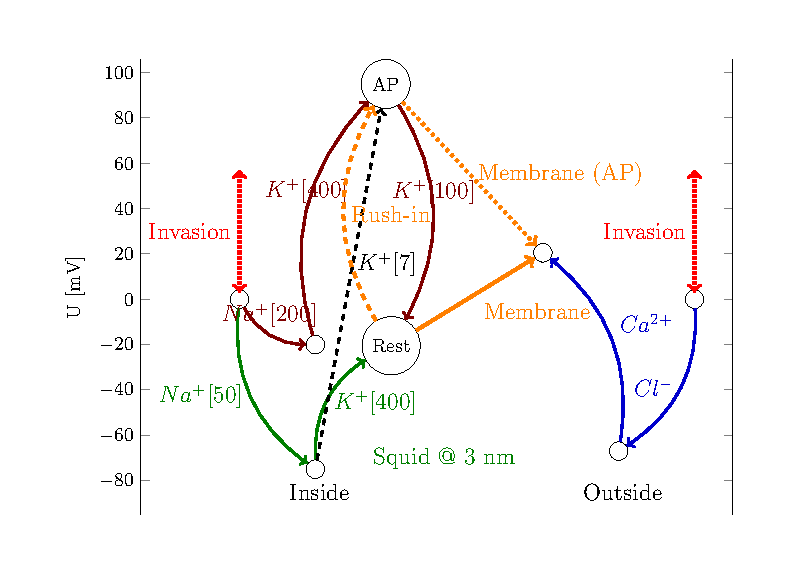
\includegraphics[width=.9\columnwidth]{fig/RestingPotential5.pdf}
	\caption{The figure is supplemented with the unbent black line showing that the clamping condition forces the neuron
		to find a new balanced state by compensating the clamping voltage
		by setting a concentration [Na50,K7].
		For comparison, the case of natural \gls{AP} is also shown.
		The mechanism of producing \gls{AP} (using numbers referring to the case of squid shown in Table~1 in~\cite{VeghUnifiedCrossdisciplinaryModel:2026}). In the resting state, the inside thermal potentials follow the green paths.
		When the rush-in of $Na^+$ ions suddenly increases the internal concentration to $[200]$, the potential on the internal side of the membrane increases to $+90\ mV$. The neuron must decrease its concentrations to restore the resting potential, mainly by releasing an action potential through the \gls{AIS}.
		The clamping fixes the neuron's membrane voltage at \gls{AP},
		so the neuron can operate only with the concentrations.
		\label{fig:RestingPotential5}
	}
\end{figure}
\else
begin{figure}
\centering
	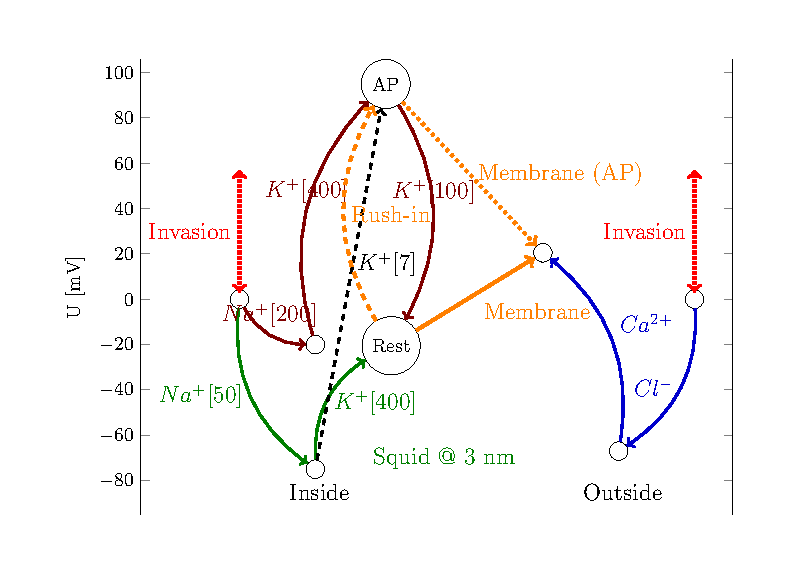
\includegraphics[width=.9\columnwidth]{fig/RestingPotential5.pdf}
	\caption{The figure is supplemented with the unbent black line showing that the clamping condition forces the neuron
		to find a new balanced state by compensating the clamping voltage
		by setting a concentration [Na50,K7].
		For comparison, the case of natural \gls{AP} is also shown.
		The mechanism of producing \gls{AP} (using numbers referring to the case of squid shown in Table~1 in~\cite{VeghUnifiedCrossdisciplinaryModel:2026}). In the resting state, the inside thermal potentials follow the green paths.
		When the rush-in of $Na^+$ ions suddenly increases the internal concentration to $[200]$, the potential on the internal side of the membrane increases to $+90\ mV$. The neuron must decrease its concentrations to restore the resting potential, mainly by releasing an action potential through the \gls{AIS}.
		The clamping fixes the neuron's membrane voltage at \gls{AP},
		so the neuron can operate only with the concentrations.
		\label{fig:RestingPotential5}
	}
\end{figure}
\fi



\renewcommand{\arraystretch}{1.3}
\begin{table}
	\caption{The summary data table for equilibrium (Data from Table 2.1 in~\cite{JohnstonWuNeurophysiology:1995}. For the graphic representation 
	of potential balance see Figure~\ref{fig:RestingPotential3} ) \label{Tab:SummaryTable}}
\iflatexml	
	\begin{tabular}{ |p{0.6cm}||p{0.9cm}|p{1.05cm}|p{3.9cm}| p{1cm}| p{1cm}| p{1.1cm}|}
	\else
	\begin{tabular}{ |p{0.55cm}||p{0.65cm}|p{0.65cm}|p{3.38cm}| p{1.1cm}| p{1.1cm}| p{1.1cm}|}
	\fi
	\hline
	\hline
 Ion& [In] &[Out] &  $U_{therm}\frac{RT}{zF} log\bigl( \frac{[C]_{o}}{[C]_{i}}\bigr)$ &$U_{electr}^{theor}$&$U_{electr}^{exper}$&$U_{membr}$\\
	& [mM] & [mM] &  [mV] &  [mV] &[mV]&[mV]\\
	\hline
&\multicolumn{6}{|c|}{Squid \cite{HodgkinHuxley:1952} \  T=293\ $K^o$ \  Width= \textbf{3}\ [nm] \  Field= \textbf{14.0}\ [MV/m] 
}\\
	\hline
\em	$K^+$ & 400 & 20 & $-75.5= 58 log\bigl( \frac{20}{400}\bigr)$& \textbf{41.9}&\textbf{41.4}&-62.0\\
	$Na^+$ & 50 & 440 & $+54.8= 58 log\bigl( \frac{440}{50}\bigr)$&&&\\
	$Cl^-$ & 40 & 560 & $-66.5= 58 log\bigl( \frac{560}{40}\bigr)$&\textbf{41.9}&\textbf{42.0}&63.0\\
$Ca^{2+}$ & $0.27^*$ & 10 & $+45.5= 29 log\bigl( \frac{10}{0.27}\bigr)$&&&\\
&\multicolumn{6}{|l|}{$^*$ used for the published value 0.4} \\

	\hline
&\multicolumn{6}{|c|}{Frog muscle (Conway) \  T=293\ $K^o$ \  W = \textbf{8}\ [nm] 
\  E= \textbf{9.6}\ [MV/m] 
}\\
	\hline
$K^+$ & 124 & 2.25 & $-101= 58 log\bigl( \frac{2.25}{124}\bigr)$&\textbf{88.9}&\textbf{83.6}&-125.4\\
$Na^+$ & 10.4 & 109 & $+59.2= 58 log\bigl( \frac{109}{10.4}\bigr)$&&&\\
$Cl^-$ & 1.5 & 77.5 & $-99.4= -58 log\bigl( \frac{77.5}{1.5}\bigr)$&\textbf{88.9}&\textbf{82.7}&124.1\\
$Ca^{2+}$ & $0.021^*$ & 2.1 & $+58.0= 29 log\bigl( \frac{2.5}{0.25}\bigr)$&&&\\
&\multicolumn{6}{|l|}{$^*$ used for the published value 4.9} \\

	\hline
&\multicolumn{6}{|c|}{Mammalian cell \  T=310\ $K^o$ \  W= \textbf{6}\ [nm] 
\  E= \textbf{11.1}\ [MV/m] 
}\\
	\hline
$K^+$ & 140 & 5 & $-89.7= 62 log\bigl( \frac{5}{140}\bigr)$&\textbf{57.7}&\textbf{57.3}&-85.8\\
$Na^+$ & 15 & 145 & $+61.1= 62 log\bigl( \frac{145}{15}\bigr)$&&&\\
$Cl^-$ & 4 & 110 & $-89.2= -62 log\bigl( \frac{110}{4}\bigr)$&\textbf{57.7}&\textbf{56.9}&85.9\\
$Ca^{2+}$ & $0.04^*$ & 5 & $+60.8= 31 log\bigl( \frac{5}{0.04}\bigr)$&&&\\
&\multicolumn{6}{|l|}{$^*$ used for the published value 0.0001} \\

	\hline
&\multicolumn{6}{|c|}{$Na^+$ ions only~\cite{OriginMembranePotential:2018}\ T=310\ $K^o$ \  W= \textbf{6}\ [nm]
\ E = \textbf{10.0}\ [MV/m] 
}\\
	\hline
$Na^+$ & 12 &145 &$+66.6= 62 log\bigl( \frac{145}{12}\bigr)$&60.7&66.6&\\
	\hline
	\hline
\end{tabular}
\end{table}


\ifx\magyar\undefined
\section[Describing clamping]{Describing invasion: clamping\label{sec:V2-0_ElectricClamping}}
\else
\section[Feszültségrögzítés leírása]{Feszültségrögzítés leírása\label{sec:V2-0_ElectricClamping}}
\fi

\ifx\magyar\undefined

\else
A \hyperlink{phys:ElectricModel}{\ref{phys:ElectricModel} physics panel}
magyarázata szerint 
\fi

\section[The outward K+ component during the Action Potential]
{The outward K+ component during the Action Potential\label{sec:Fallacies-OutwardK}}

Emitting Action Potentials is a fundamental aspect of neuronal operation.
\gls{HH} hypothesized that neurons operate with electrical currents and 
suggested the idea~\cite{HodgkinHuxley:1952} that the neuronal operation
is more or less reminiscent of an electric oscillator. Given that the parallel $RC$ circuit they hypothesized cannot produce an output voltage with opposite sign, they had to introduce
the concept of a delayed current in the opposite direction. Even, they demonstrated that $K^+$ current flows in the second half 
of the \gls{AP}. The net electrical model led immediately to contradiction with the empirical evidence that, 
as Hodgkin wrote~\cite{HodgkinConduction:1964}, "Hill and his colleagues found~\cite{HeatProductionNeuron:1958} that an initial phase [of the action potential] was followed by one of
heat absorption. [...] a net cooling on open-circuit was totally unexpected
and has so far received no satisfactory explanation."
Not to mention the mechanical, optical, etc. effects~\cite{MechanicalWaves:2015}; accompanied by \gls{AP}. 
Neglecting the \gls{AIS} and sticking to \gls{AIS}-less model 
led to clue-less ad-hoc assumptions and desperate claims such as 
"The sodium influx associated with
depolarization is exothermic  [...] the capacitive energy stored in the membrane is
released as heat. However, the efflux of $K^+$  ions is endothermic [...] \textit{converting heat in the environment
into capacitive energy at the membrane}."~\cite{MechanicalWaves:2015}
(That anti-dissipation effect would be something new for physics and could convert the harmful global warming to an
inexhaustible energy source for humankind.)
The correct physical explanation can be derived using the 
unified model of neuronal operation~\cite{Vegh2025ThermodynamicModel:2026,VeghUnifiedCrossdisciplinaryModel:2026}: under the mechanical pressure
caused by the mutual repulsion of the ions, the electrolyte
is compressed and expanded.

One of the big mysteries in the creation of the V1.0  model was why \gls{AP}
became negative when only
$Na^+$ influx was seen when \gls{AP} was formed. 
Given that they found only positive charges nearby, they supposed that
an outflux of positive charges, namely of $K^+$ ions,  was the reason.
Since the process is too fast, \gls{HH} used a voltage clamping method for the experimental demonstration~\cite{HodgkinHuxleyCurrent:1952} of the hypothesized  $K^+$ current. The essence of this is that they
imitated the crossing of the membrane voltage threshold (reaching the "AP" state, see Fig.~\ref{fig:ClampingKCurrent}):
"(after completion of the quick pulse through the membrane
capacity)", then raised the intracellular domain of the membrane to a potential higher than the resting potential with a negative feedback circuit:
"the potential
difference across the membrane is suddenly changed from its resting
value, and held at the new level by a feed-back circuit ('voltage clamp' procedure)", and measured the time dependence of the current in this state.

\subsection[The formal description of the process]
{The formal description of the process\label{sec:Fallacies-OutwardKPhysicsFormal}}

Figure \ref{fig:RestingPotential5} shows the changes that occur in a neuron that is displaced from its equilibrium state.
These processes are naturally slow, their role in the
transient process is discussed in the \ref{sec:TransientState} section,
here we only illustrate our statements regarding the $K^+$ current.
Our statement is essentially based on Kirchhoff's Voltage Law,
according to which the sum of the voltages in a closed circuit is zero.
 In our case, the circuit extends from the inside of the neuron to the external environment.
If for any reason the external and internal potential levels are not the same, then a current flows until they are equalized (current carries charge and causes a potential change; it is not an ideal voltage generator).
Of course, the equalization is not
instantaneous, the current has a time dependence.

On both the left and right sides of the figure, the resting potential level is
at the zero value of the vertical scale. In the resting state (without invasion),
in the intracellular segment
the [Na50,K400] concentrations are present inside the cell. Using these values, we reach the "Rest"
state along the green arrows (based on the Nernst voltages, see \ref{Tab:SummaryTable}~Table), which is located at a height of \SI{-21}{\milli\volt}.
On the right side, in the extracellular segment, from the point also at a height of 0, we arrive at a point at a height of \SI{21}{\milli\volt} along the blue arrows in the same way. The potential difference between the two mentioned points is \SI{42.5}{\milli\volt}, which \gls{HH} measured. It is a correct value,
but it is the result of an electrostatic charging and not of a voltage drop due to the "leakage current" they assumed.
\index{leakage current}
The voltage across the membrane (represented by the solid orange arrow) points upwards, preventing positive ions in the intracellular space from moving towards the extracellular space and preventing negative ions in the extracellular space from moving towards the intracellular space. The $Ca^{2+}$ ions in the extracellular segment, however, are permeable, requiring continuous pumping. There is no potential difference between the outside and inside, so no (significant) current flows.

If, for any reason, the membrane voltage suddenly rises above the threshold value, due to the extremely fast $Na^+$ influx,
the membrane potential increases by about \SI{100}{\milli\volt} (a [Na200,K400] state occurs, see the brown arrows), i.e. the neuron jumps into the AP bubble.
%After the threshold is exceeded naturally or with a short pulse, the "AP" passes into the "Rest" bubble,
%this is the same in the case of natural and clamping measurements.
The orange arrow that was pointing upwards now points downwards as a broken line: the outflow of positive ions (both $K^+$ and $Na^+$) is given a free path, but the sloping path for $Ca^{2+}$ ions is eliminated. However, the free ions in the surface layer of the membrane are the vast majority of the $Na^+$ ions that have just arrived, so the ion current through the \gls{AIS} mainly consists of such ions.
A significant increase in the membrane voltage leads to a significant increase in the potential of the
inner space of the neuron.
A current is initiated that tries to restore the initial voltage and concentration relationships.
The extracellular environment of the membrane is extremely stable (the concentrations do not change),
but inside the cell the voltage increases to the same extent, in the direction of "Invasion".
The membrane potential has changed significantly due to the change in the $Na^+$ concentration, so the cell then moves them towards equilibrium.


In the case of natural \gls{AP}, there is no obstacle for the neuron
to restore its previous state by changing any parameter, so the system concentrations
start towards the state [Na50,K400]. This can be
easily achieved by trying to make Na[50] from Na[200], while $K^+$ is still/already at the appropriate concentration.
That is, it releases (mainly) $Na^+$ ions through the \gls{AIS} until the potential difference drops to zero.
Reducing the $Na^+$ concentration also reduces the membrane
voltage, i.e. after the release of the excess ions (admitted during the $Na^+$ rush-in) the neuron returns to its initial state;
a cycle takes place.

"Clamping" fixes the membrane voltage, meaning that the neuron cannot restore its initial
resting state. Instead, it has to find a new balance by changing the concentrations.
After the artificial \gls{AP}, clamping (using a negative feedback) keeps the membrane potential at a fixed value, so the neuron can only produce a new balance by changing the ion concentrations: a current flows until the Nernst voltages of the $Na^+$ and $K^+$ concentrations can balance the clamping voltage.
From this [Na50,K400] state, the neuron has to adjust the potential so that the sum of the Nernst voltages plus the membrane's voltage plus the clamping voltage is zero (so another balance has to be set!), while the voltage is fixed.
To do this, it must reduce the $K^+$ concentration, while the $Na^+$ concentration is already at a good value (the opposite of the previous case). And not by a small amount: [K7] only causes a voltage change equal to the clamping 100 mV imposed on the cell.
This voltage is given by the green curved $Na^+[50]$ and the black dashed straight
$K^+[7]$ path. The neuron can achieve this [Na50,K7] concentration
by starting an intensive $K^+$ release.

\begin{figure}
\centering
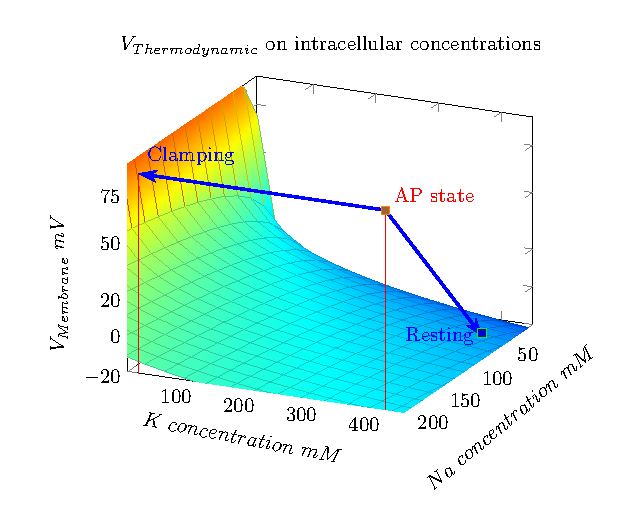
\includegraphics[width=.9\columnwidth]{fig/ClampingKCurrent.pdf}
\caption{Artificial and natural degradation of the AP state.
In the case of natural degradation, the neuron
has to get rid of the (unnecessary) $Na^+$ ions;
by releasing them, it returns to the initial state;
cycle takes place.
Clamping keeps the membrane voltage fixed,
so the neuron can only establish a new equilibrium situation by changing the intracellular concentrations
which, due to the very reduced $K^+$ concentration, is only possible with an intense
$K^+$ release.
\label{fig:ClampingKCurrent}
}
\end{figure}

Another important difference compared to the natural case is that there is no electrostatic acceleration across the membrane (which is why the $Na^+$ influx stopped),
only a thermodynamic suction effect outwards due to clamping.
Indeed, $K^+$ ions attempt flow out through the membrane, but
they cannot exit until the electric potential drops
below the equivalent thermodynamic driving force of the concentration.
Moreover, the nearby $K^+$ ions get there sooner, but they leave a gap (reduced concentration) behind them, where the nearby neighbor $K^+$ electrodiffuses. This is why the physiologist sees a "delayed current".
It is a strange game of nature that the resultant of the thermodynamic and the electric  (plus the elastic)  gradients moves, simultaneously, the $Na+$ ions parallel to the membrane surface, toward the \gls{AIS}, and
the $K^+$ ions perpendicular to the surface toward the membrane,
approximately until the peak of the action potential voltage is reached.
The $Na^+$ starts to leave through the \gls{AIS}, while the "excessive" $K^+$ ions leave through the membrane.
\textit{The two currents do not flow in the same path, so they cannot
interfere as currents in opposite directions and cannot cause hyperpolarization.}
\index{hyperpolarization}
Hyperpolarization is caused by the reversal of the $Na^+$ current, which can be interpreted
in the electrical sense as the capacitive current of the capacitor in the serial $RC$ circuit, and
in the mechanical sense as the negative period of the elastic membrane oscillation.

\textit{That is, the $K^+$ current is an artifact caused by the clamping, which is caused by the 'clamping' measurement conditions, and does not occur in the neuron under natural conditions.}


So, this is where the urban legend "$K^+$ flows out through the membrane in the second phase of \gls{AP}, with a significant delay compared to the $Na^+$ influx" comes from.
It is really a real measurement, it is really $K^+$ ion, but they did not measure what they thought.
\gls{HH} and their late descendants did too. So there is no question of specific $Na^+$ and $K^+$ (synchronized with each other) channels: in both cases, the concentration and potential relationships decide what ions flow and in which direction.
%It doesn't hurt to use a good model for what you want to study.
\gls{HH} was aware that theirs was not good, but they didn't know any better.
Unfortunately, they spread the misconception.



In the classic experiment of \gls{HH}, clamping means that the left-hand "Invasion" suddenly raises the membrane voltage to the peak value measured at \gls{AP}, without the concentrations changing, so the voltage of the left-hand segment will also be higher.
The current only stops when the difference in the Nernst voltages of the inner segments equalizes
the clamping voltage. Due to the slowness of charge carriers, the process is not instantaneous.

Fig.~\ref{fig:ClampingKCurrent} shows a pictorial summary of the process. The points on the surface give the Nernst voltage acting on the ions, for different combinations. The points on the surface are in equilibrium. The onset of the \gls{AP} moves the point that was in equilibrium until then well outside the surface. The neuron can find the new equilibrium position without the forcing effect of clamping by restoring the parameters of the previous state. In the case of clamping, it must set new concentrations at which the sum of the Nernst voltages can counteract the clamping voltage. In both cases, a relaxation process takes place, which in the case of the native process is measured by physiology as \gls{AP}.

% Compiled 26.07.10
\subsection[The physics of the process]
{The physics of the process\label{sec:Fallacies-OutwardKPhysics}}

The essential functioning of the cell largely takes place in layers of a few nanometers close to the cell membrane, where differences in concentration and voltage gradients (and consequently material flow rates) of up to several orders of magnitude can occur for a few dozen microseconds. Furthermore, the slow material flow creates potential and concentration changes that change from moment to moment, and whose effects can be significantly different in each layer due to the chemical quality of the ions. For this reason, the description of the events is unique in each case, for each layer and for each time period; it is not uncommon for scientific disciplines to be changed when describing individual stages, or for them to be combined in a different way.

The two ends of the ion channels embedded in the membrane have different potentials and concentrations, so that the ions passing through acquire significant energy and speed. However, this gradient disappears when they exit the channel, so that the ions "stop" in frustration. The passage continues until the passing ions increase the electrochemical potential of the other side so much that the gradient disappears. Inside the electrolyte, the other, orders of magnitude smaller gradients continue to operate, of course, but can only create very slow material transport. The changes in the "bulk" part of the electrolyte tend towards slow equalization (different rules remain in effect near the boundary membrane). For this reason, a slow diffusion effect is also associated with all processes.

When $Na^+$ ions penetrate the intracellular segment, they do so under the influence of a significant electrochemical gradient. In this way, immediately after the passage (lasting a few nanoseconds), the ions create a $Na^+$-rich layer, from which the charge of the ions (partly by direct collision) knocks out the ions there, mainly $K^+$.
Basically, a $Na^+$ layer is formed directly under the intracellular part of the membrane, which increases the voltage on the capacitor plates, and since the \gls{AIS} at the end of the membrane acts as a sink for the ion current, an immediate $Na^+$ current is initiated, as discussed in the electrical model.
$Na^+$ ions move along the membrane surface due to the high electrical gradient through the high-conductivity \gls{AIS}, but small amounts of $Na^+$ and $K^+$ ions apparently diffuse into the adjacent layer. The ion concentration and potential of the layer decrease with the outflow current. Due to the slowness of the ion current, the ions only reach the \gls{AIS} in tens of microseconds.
The membrane is initially closed to positive ions (after the $Na^+$ ions have passed through), and the $Na^+$ layer represents an additional potential barrier. However, over time, the decreasing $Na^+$ concentration due to the current in the layer that causes the \gls{AP} increasingly allows $K^+$ ions to move towards the membrane and the experienced $K^+$ current to start, which is only possible after a few dozen microseconds.

"Delayed $K^+$ channels" therefore mean ion channels that structurally do not distinguish between ions, and the delay is caused by transient processes taking place in the ion layers. These channels indeed release $K^+$ ions, which only start when the clamping voltage is switched on to the neuron (i.e., they create a non-equilibrium state of the neuron segment), and only $K^+$ ions because the thermodynamic gradient is only favorable to them.

\gls{HH} found that the \gls{AP} can be decomposed into two currents:
"the ionic current during a depolarization consists of two more or less independent components in parallel, an early transient phase of current carried by sodium ions, and a delayed long-lasting phase of current carried by potassium ions".
Their conclusion is more than surprising, that although the current component arising from Na ions appears quickly, the component consisting of $K^+$ ions remains delayed and persistent. According to that "explanation", the neurons are disposable devices: after emitting a single \gls{AP}, the neuron emits a short-lasting $Na^+$ and (according to their figures 5 and 6) an infinitely long-lasting $K^+$ current, contrary to experience.
In other words, for \SI{100}{\pico\ampere} (that is \SI{1e-10}{\ampere}) saturation current and \SI{1e11}{neuron} it would mean
10~amper permanent current in the brain.
Furthermore, it would keep the resting potential above 
the value of the resting potential. The difference 
would be the extra voltage of the clamping; that is,
it would disappear at zero claping voltage.
In other words, the extra voltage and the  $K^+$ current disappears in the absence of clamping, as observed.

In our reading the current lasts as long as the voltage invasion caused by clamping persists or the $K^+$ content of the intracellular segment of the neuron is depleted.


